\documentclass[../main]{subfiles}
\begin{document}
\chapter{Flutter}

In this chapter, the first an introduction to structural wind engineering is provided and is extended to flutter. Then flutter mechanism and 
methods to obtain flutter derivatives are discussed. Then the mathematical formulation for calculating the critical wind speed is provided. 
Finally, the multi-frequency method is introduced and its workflow is compared with the single-frequency method.

% ─────────────────────────────────────────────────────────────────────────────

\section{Structural Wind Engineering}
Structural wind engineering can be viewed as a field in civil engineering studying how a structure will respond when wind passes over through it. 
This is studied by combining the concepts of fluid mechanics and structural mechanics to understand the mechanisms of different response and quantify the load due to it.
Response of a structure for a wind load can broadly be classified into two types. 1. Along wind response and 2. Across wind response. 
Along wind responses are the force (due to wind) acting on the structure in parallel to the direction of wind. And in across wind response, this force
is perpendicular to the direction of wind. Also since wind is a time varying load, the response of the structure to the wind load is dynamic in nature. 
So analysis of structure subjected to wind needs to be differentiated between static and dynamic analysis. In static analysis, the response of the structure is 
due to the mean wind load is analysed. And in dynamic analysis, the response of the structure is due to the fluctuating component (time varying) 
of the wind load is considered. The primary source of static is along wind reponse created due to drag force excerted by the wind structure. 
The major source of dynamic wind loads are response due to buffeting, vortex induced vibration and movement induced vibration. 

Buffeting is along wind response caused by turbulence in the wind. This shall be understood as, if we plot
a graph between wind velocity vs time, then the mean of thiswind velocity is the static component  and the variance
of this plot is the buffeting component. The calculation of buffeting component is given EN 1991-1-4. 

Next, Vortex induced vibration (VIV) is an across wind response that occurs in a bluff body. This is caused due to the alternate shedding of 
vortices in the wake region of the structure. A bluff body shall be understood as an object that disturbs the streamline flow of a fluid and casuing seperation
points. Wake is the region in the downstream of the body where the flow is highly disturbed and has negative pressures. When the fluid flows around an object,
the flow seperates at the seperation points and forms wake region in the downstream. When the velocity (reynolds number) of the fluid is low, the vortex will time 
invariant and the structure will be subjected to a constant along wind force, that is static and buffeting response. But if the velocity is high, the flow becomes unstable causing the vortices 
to shed alternately from the two sides of the structure. This induces an alternating time varying force of sinosoidal manner in accross wind direction. 
This causes vibration to the strcuture known as vortex induced vibration. Since this is a dynamic force, it imposes greater attention to calculation 
of the frequency of the force as this can decide on resonsce of our building. When the frequency of vortex shedding matches with the 
natural frequency of the structure, it can cause resonance leading to large amplitude vibrations and potential structural failure.
The voretx shedding frequency is given by the formula f = St*U/D, where D is the characteristic length of the structure and U is the velocity of the fluid. 
St is the non dimensional parameter called Strouhal number, which is a shape constant. For regular shapes, the value of St shall be taken from EN 1994-1-4.   

Finally, movement induced vibrations are caused due to the interacition between the wind and the structure. When a wind passes through a structure, 
it creates a force that cause deformation/displcement in the strcuture. Now due to this displacement, 
the flow around the strcuture changes and consequently the force acting on the structure changes (also depending on the rate of change of displacement). This can create a positive feedback loop where the 
deformation causes an increase in the force, which in turn causes more deformation. This can lead to a rapid increase in the amplitude of vibrations, which can 
ultimately result in structural failure. Flutter and galloping are the examples of this type of dynamic instability. Torsional divergence is also this type of instability excpet 
this stability is static in nature. This can be observed in failure of solar panels, etc. 

These phenomena are known as movement induced vibration first an initial motion is required to trigger this phenomenon to start. 
This indicates loss in any one of the structural parameters such as stiffness, damping, etc due to the interaction with wind. In torsional
divergence, stiffness of the structure is lost due to interaction with wind and in flutter, the loss is damping. Since flutter is 
the focus of this thesis, the following sections will be focued on discussing the mathematical formulations for quantifying this loss.
Also before starting the discussion on flutter, first galloping is discussed. This is done because, galloping is a similar phenomenon to flutter with lesser complexity 
and hence it can be useful in intuitive understanding of these aeroelastic phenomena.

\section{Galloping}

Consider a 1-DOF spring-mass system with a bluff body attached to it. When the wind passes through the bluff body, it creates a drag and lift force. 
Assume, due to an external forced vibration or VIV, the stucture starts to vibrate in the vertical direction. Now, due to this vertical motion, 
the angle of attack of the wind on the bluff body changes. %This is because a body under rest and in motion will not experience same force vector. 
Since the angle of attack changes, the lift and drag forces also change (except for section where for any angle of attack the lift force remains constant - like circle).
If the change in lift force is such that it increases the motion amplitude, then a positive feedback loop is created. This is known as galloping. 
This is the reason behind a pure circular rope or cable will not undergo galloping, as the lift force is zero for all angle of attack. 
But a rectangular section will undergo galloping as the lift force changes with angle of attack.

Here, the necessary condition for galloping is that the change in lift force with respect to angle of attack should be positive.

The lift force acting on the structure can be given by the equation,
% Equation (15.18)
\begin{equation}
L_{\mathrm{ae}}(\alpha) = \frac{\rho_{\mathrm{air}}\,v_{\mathrm{wind}}^2}{2}\,d\,c_L(\alpha) %= q\,d\,c_L(\alpha) 
\end{equation}

where, $\rho_{\mathrm{air}}$ is the density of air, \\
$v_{\mathrm{wind}}$ is the velocity of wind, \\
$d$ is the characteristic length of the structure \\
and $c_L(\alpha)$ is the lift coefficient as a function of angle of attack $\alpha$ (Figure \ref{fig:galloping}). \\

Now, the equation of motion for the system can be written as,

\begin{equation}
m\,\ddot{w} + c\,\dot{w} + k\,w = L_{\mathrm{ae}}(\alpha) = \frac{\rho_{\mathrm{air}}\,v_{\mathrm{wind}}^2}{2}\,d\,c_L(\alpha)
\end{equation}

To solve the equation, we can linearise the lift force by assuming small angle of attack, which gives us the following equations,
\begin{equation}
L_{\mathrm{ae}}(\alpha) \approx \left.\frac{\mathrm{d}c_L}{\mathrm{d}\alpha}\right|_{\alpha=0}\alpha\,q\,d
\end{equation}

\begin{equation}
\alpha \approx \tan\alpha = \frac{\dot{w}}{v_{\mathrm{wind}}}
\end{equation}

Substituting these into the equation of motion, we get

% Equation (15.22)
\begin{equation}
m\,\ddot{w} + c\,\dot{w} + k\,w = \left.\frac{\mathrm{d}c_L}{\mathrm{d}\alpha}\right|_{\alpha=0}\frac{\dot{w}}{v_{\mathrm{wind}}}\frac{\rho\,v_{\mathrm{wind}}^2}{2}\,d
\end{equation}

% Equation (15.23)
\begin{equation}
m\,\ddot{w} + \left(c - \left.\frac{\mathrm{d}c_L}{\mathrm{d}\alpha}\right|_{\alpha=0}\frac{\rho\,v_{\mathrm{wind}}\,d}{2}\right)\dot{w} + k\,w = 0
\end{equation}

Here we can see how the system damping is affected by the interaction with wind: Effective damping = $c - \left.\frac{\mathrm{d}c_L}{\mathrm{d}\alpha}\right|_{\alpha=0}\frac{\rho\,v_{\mathrm{wind}}\,d}{2}$. 
When this effective damping becomes negative, the system becomes unstable and galloping occurs. 
Hence, the critical wind speed for galloping can be obtained by setting the effective damping to zero, which yields,

% Equation (15.24)
\begin{equation}
v_{\mathrm{crit}} = \frac{2c}{\left.\frac{\mathrm{d}c_L}{\mathrm{d}\alpha}\right|_{\alpha=0}\rho\,d}
\end{equation}

\begin{figure}[htbp]
    \centering
    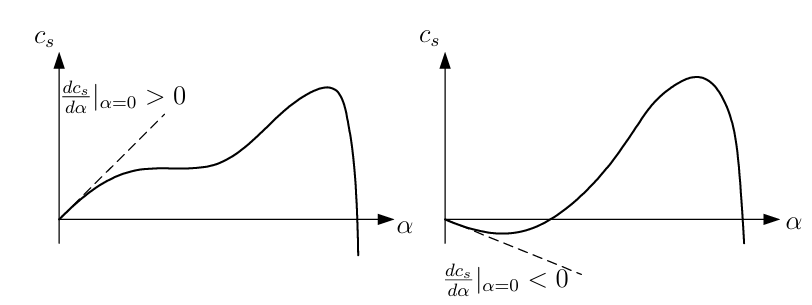
\includegraphics[width=1\textwidth]{Figures/Galloping_2.png}
    \caption{}
    \label{fig:galloping}
\end{figure}


\section{Flutter Analysis}

Flutter is a dynamic instability phenomenon that occurs when the aerodynamic forces acting on a structure couple with its natural modes of vibration, leading to self-excited oscillations.
Consider a 2-DOF system of vertical (heave) and rotational (pitch) motion Figure \ref{fig:flutter_1}. If the vertical and pitch motion are coupled in such a way that the aerodynamic forces 
due to the vertical motion cause an increase in the pitch motion, and the aerodynamic forces due to the pitch motion cause an increase in the vertical motion, then a positive feedback loop is 
created. This can lead to a rapid increase in the amplitude of oscillations, which can ultimately result in structural failure.

\begin{figure}[htbp]
    \centering
    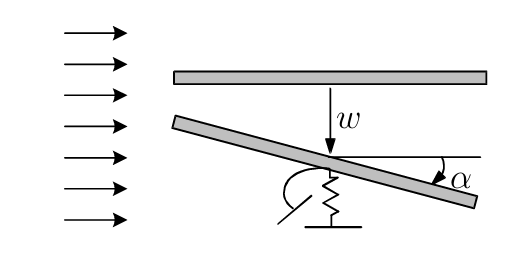
\includegraphics[width=0.5\textwidth]{Figures/Flutter_1.png}
    \caption{Two degree of freedom system for flutter analysis.}
    \label{fig:flutter_1}
\end{figure}


This is explained in figure \ref{fig:flutter_2}. Here, in the first image, it shall be observed, that the phase between the vertical and pitch motion is such that the possitive work created during the
upward motion is cancelled by the negative work created during the downward motion. Hence, the system is stable. But in the second image, the phase between the vertical and pitch motion is such that 
the positive works are created during both the upward and downward motion. Hence, a positive feedback loop is created and the system becomes unstable.

\begin{figure}[htbp]
    \centering
    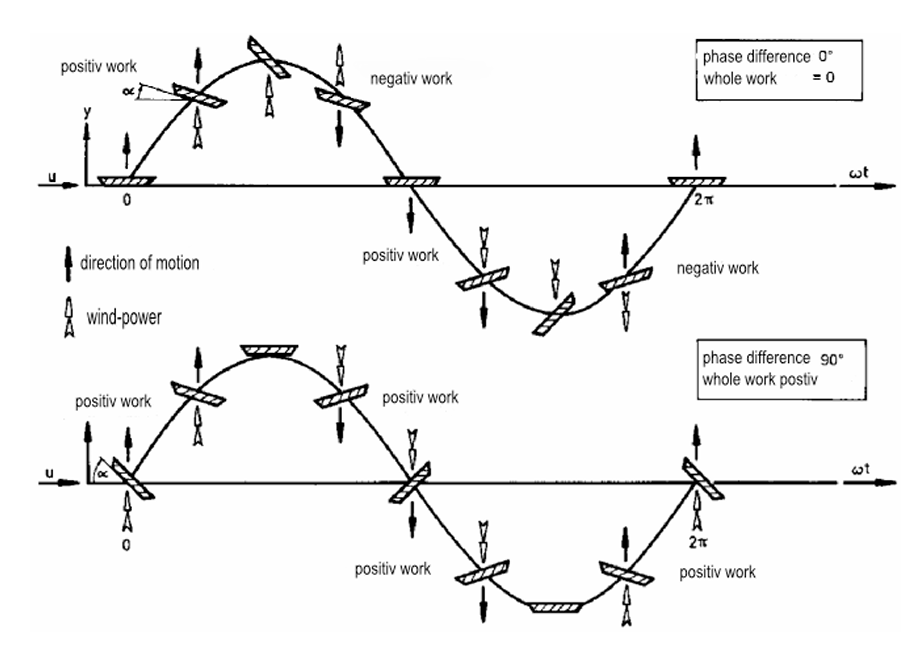
\includegraphics[width=0.75\textwidth]{Figures/Flutter_2.png}
    \caption{Flutter mechanism}
    \label{fig:flutter_2}
\end{figure}

Flutter analysis is primarily determining the critical wind speed at which this instability initiates. To do this, an dynamic equilibrium equation is solved considering aerodynamic forces. 
The dynamic equilibrium equation for a 2-DOF system is


\begin{align}
\label{eq:eq_of_motion_h}
m(\ddot{h} + 2\omega_h\xi_h\dot{h} + \omega_h^2 h) = L_{ae} \\
\label{eq:eq_of_motion_alpha}
I_\alpha( \ddot{\alpha} + 2\omega_\alpha\xi_\alpha\dot{\alpha} + \omega_\alpha^2 \alpha) = M_{ae} 
\end{align}

where, $L_{ae}$ - Aerodynamic lift force due to wind \\
\phantom{where,} $M_{ae}$ - Aerodynamic moment due to wind
\vspace{0.5 cm}

Here, quantifying the aerodynamic forces is the challenge. In 1934, Theodorsen, a Norwegian American aerodynamicist, developed an 
analytical solution for the aerodynamic forces for unsteady flutter analysis of an airfoil \cite{TheodorsenGarrick1934}. The solutions for $L_{ae}$ and 
$M_{ae}$ were functions of theodorsen circulatory functions, which, in turn, are functions of $K$, the reduced frequency, where 
$K = \frac{\omega b}{U}$. This quantifies the unsteadiness (i.e., the time lag between the applied force and the structure's 
displacement). As this theory was based on the assumption of Potential flow, it cannot be applied to bridges. In 1971, Scanlan, 
an American civil engineer, reformulated Theodorsen's theory to accommodate bridges using a semi-empirical method based on eight 
functions (for a 2-DOF system) known as flutter derivatives \cite{scanlan1971}.

\begin{equation}
\label{eq:lift_force}
L_{ae} = \frac{1}{2}\rho U^2 B \left[ KH_1^* \frac{\dot{h}}{U} + KH_2^* \frac{B\dot{\alpha}}{U} + K^2 H_3^* \alpha + K^2 H_4^* \frac{h}{B} \right]
\end{equation}

\begin{equation}
\label{eq:moment_force}
M_{ae} = \frac{1}{2}\rho U^2 B^2 \left[ KA_1^* \frac{\dot{h}}{U} + KA_2^* \frac{B\dot{\alpha}}{U} + K^2 A_3^* \alpha + K^2 A_4^* \frac{h}{B} \right]
\end{equation}

where, $h$ - vertical DOF (Heave motion), $\alpha$ - Rotational DOF (Pitch Motion)\\
\phantom{where,} $H_1^*, H_2^*, H_3^*, H_4^*, A_1^*, A_2^*, A_3^*, A_4^*$ are flutter derivatives\\

Flutter derivatives are shape constants that quantify the wind force on a structure as a linear relation 
of the section's vertical velocity, angular rotation, and speed of angular rotation. They are inturn functions 
of $U_{red} = \frac{1}{K} = \frac{U}{fB}$. This shall be viewed as: how $C_d$, acts as a non-dimesional shape constant for computing dgrag force on a strcuture, 
each of the flutter derivatives is for quantifying the aerodynamic lift and moment forces. For example, 
$H_1^*$ is the flutter derivative for quantifying the lift force due to vertical velocity of the structure. $A3^*$ is 
the flutter derivative for quantifying the moment force due to angular rotation of the structure.

These flutter derivatives should be found through external CFD simulations or wind-tunnel tests. 
Once found this is applied back to the dynamic equilibrium equation to find the critical velocity.
The approaches for finding the Flutter Derivatives can be broadly classified based on 
the nature of the applied motion (Free vibration or forced motion). In forced motion tests, the structure is forced to 
oscillate at a specific frequency and amplitude, and the resulting aerodynamic forces are measured to determine the flutter derivatives.
In free vibration tests, the structure is allowed to vibrate freely under the influence of aerodynamic forces, 
and the flutter derivatives are determined from the observed damping response.
For the preliminary analysis of flutter, forced motion tests with CFD have greater 
importance due to their easier setup and lower cost. 

\section{Identification of Aerodynamic Forces with CFD}

The procedure to obtain the aerodynamic forces are obtained using forced-motion CFD simulations is explained below. 
A 2-D cross-section of the bridge deck is modelled in a virtual wind tunnel with appropriate boundary conditions. The bridge cross-section is then oscillated 
sinusoidally in the vertical (heave) direction according to
\begin{align}
    h(t)       &= h_0 \sin(\omega t), \\
    \dot{h}(t) &= \omega h_0 \cos(\omega t),
\end{align}
where $h_0$ is the maximum amplitude of the applied heave motion and $\omega$ is the angular frequency of the applied heave motion. 
Since no pitch motion is applied, $\alpha = \dot{\alpha} = 0$, and the aerodynamic lift force and pitching moment simplify to
\begin{align}
    L_{ae} &= \frac{1}{2}\rho U^2 B
              \left[KH_1^*\frac{\dot{h}}{U} + K^2H_4^*\frac{h}{B}\right]
              \qquad \text{(Scanlan formulation)}, \\[4pt]
    M_{ae} &= \frac{1}{2}\rho U^2 B^2
              \left[KA_1^*\frac{\dot{h}}{U} + K^2A_4^*\frac{h}{B}\right]
              \qquad \text{(Scanlan formulation)}.
\end{align}
Under the small-amplitude assumption (small $h_0$), Scanlan's linearisation implies that the aerodynamic lift and moment 
measured from CFD take the sinusoidal form
\begin{align}
    L_{ae} &= B_0 \sin(\omega t + \phi)
           \;=\; B_1 \cos(\omega t) + B_2 \sin(\omega t), \\[4pt]
    M_{ae} &= C_0 \sin(\omega t + \Phi)
           \;=\; C_1 \cos(\omega t) + C_2 \sin(\omega t).
\end{align}

The flutter derivatives are determined by equating the lift force from the Scanlan formulation with the CFD result and 
matching cosine and sine coefficients, which gives
\begin{align}
    \frac{1}{2}\rho U^2 B
    \left[KH_1^* + K^2H_4^*\right]
    &= B_1 \cos(\omega t) + B_2 \sin(\omega t), \\[4pt]
    \frac{1}{2}\rho U^2 B^2
    \left[KA_1^* + K^2A_4^*\right]
    &= C_1 \cos(\omega t) + C_2 \sin(\omega t).
\end{align}
From this, the flutter derivatives for heave excitation are obtained as
\begin{align}
    H_1^* &= \frac{2B_1}{\rho\,\omega^2 B^2 h_0}, &
    H_4^* &= \frac{2B_2}{\rho\,\omega^2 B^2 h_0}, \\[4pt]
    A_1^* &= \frac{2C_1}{\rho\,\omega^2 B^3 h_0}, &
    A_4^* &= \frac{2C_2}{\rho\,\omega^2 B^3 h_0}.
\end{align}

The same procedure is repeated with pitch (torsional) excitation and the $H_2^*$, $H_3^*$, $A_2^*$, and $A_3^*$ derivatives are obtained.  

\begin{align}
H_2 &= \frac{{2B_1}}{\rho \omega^2 B^3 \theta_{0}}, &
H_3 &= \frac{{2B_2}}{\rho \omega^2 B^3 \theta_{0}}, \\[4pt]
A_2 &= \frac{{2C_1}}{\rho \omega^2 B^4 \theta_{0}}, &
A_3 &= \frac{2 C_2}{\rho \omega^2 B^4 \theta_{0}}.
\end{align}


Consequently, a total of two forced-motion simulations (one heave, one pitch) are required to obtain a complete set of eight flutter derivatives at each reduced velocity.

This is single frequency method where a heave/pitch motion of one 
frequency is applied to the structure to find the Flutter derivative. Obtaining flutter derivatives with 
this approach is highly computationally costly because of the following reasons. Since flutter 
derivatives are functions of reduced velocity, multiple CFD simulations (by varying the frequency 
of input forced motion) must be performed to obtain them. For finding each point in a set of 8 
flutter derivatives, 2 CFD simulations are required. To obtain an accurate representation of each 
flutter derivative function, we need a minimum of 6 to 8 points on the flutter derivative curve. 
Hence, a total of 16 simulations is required. Each CFD simulation will take approximately 48 hours. 
Hence, to obtain a complete set of flutter derivatives, 768 hours of simulation time are required. 


% ─────────────────────────────────────────────────────────────────────────────

\section{Multi-Frequency Method}

In the multi-frequency method, instead of applying the single-frequency forced-motion oscillation at a time and extracting the 4 flutter derivatives,
several frequencies are superposed applied simultaneously to the structure. By this way, n*4 flutter derivatives can be obtained from n simulations. 
For example, if 4 frequencies are applied simultaneously, then 16 flutter derivatives can be obtained from a single simulation.
The superimposition of multiple frequencies can be expressed as

\begin{equation}
    h(t) = \sum_{k=1}^{N} h_{0,k}\sin(\omega_k t + \phi_k).
\end{equation}

Under the assumption of aerodynamic linearity, the total aerodynamic response is
the superposition of the responses at each individual frequency. Consequently,
$N$ sets of flutter derivatives can be extracted from a single simulation by
applying a Fourier decomposition of the measured aerodynamic forces at each
frequency component $\omega_k$. \\

The procedures for calculating the flutter derivatives (Section~2) and the
critical wind speed (Section~3) are identical for both the single- and
multi-frequency methods. The only difference lies in the identification of
aerodynamic forces (Section~1), where multiple frequency components are excited
simultaneously rather than one at a time.
Figures~\ref{fig:single_freq_method} and~\ref{fig:multi_freq_method}
illustrate the workflow for the two methods. \\

\begin{figure}[htbp]
    \centering
    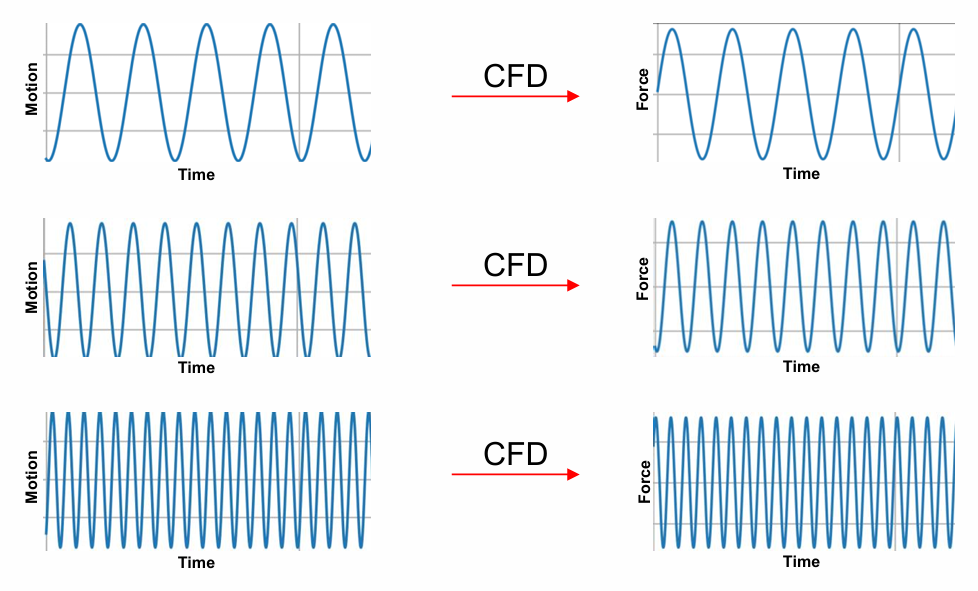
\includegraphics[width=\textwidth]{Figures/Single_Frequency.png}
    \caption{Workflow for the single-frequency method.}
    \label{fig:single_freq_method}
\end{figure}

\begin{figure}[htbp]
    \centering
    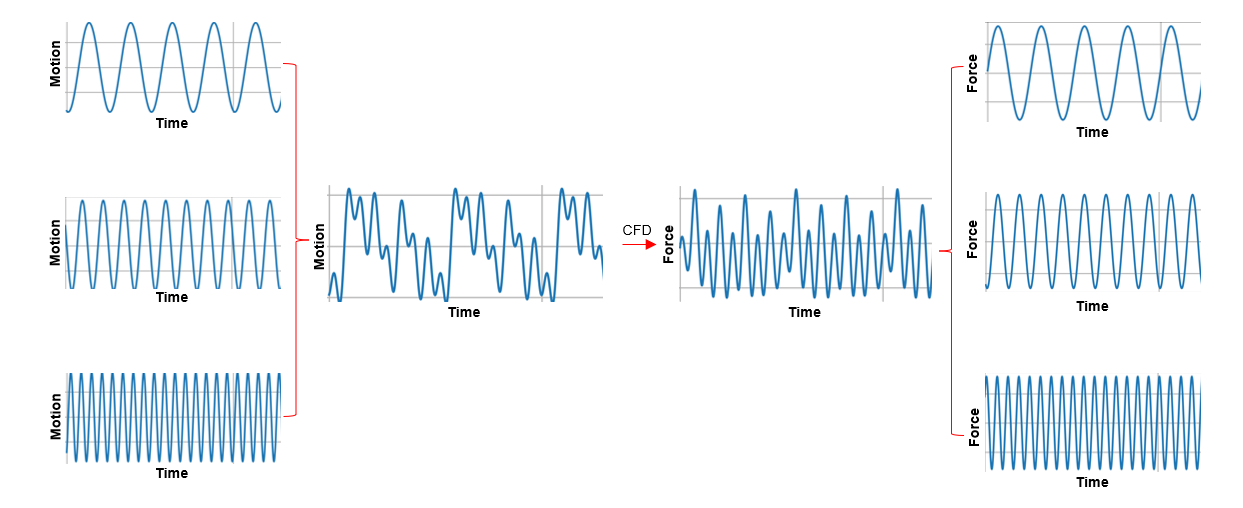
\includegraphics[angle=90, height=1.5\textwidth]{Figures/MultiFrequency_Explanation.png}
    \caption{Workflow for the multi-frequency method.}
    \label{fig:multi_freq_method}
\end{figure}


% ─────────────────────────────────────────────────────────────────────────────
\section{Calculation of Critical Wind Speed}


To obtain the critical wind speed, the equations of motion for the bridge deck (equations \ref{eq:eq_of_motion_h} and \ref{eq:eq_of_motion_alpha}) are 
equated to the aerodynamic forces from the Scanlan formulation (\ref{eq:lift_force} and \ref{eq:moment_force}) and solved.
On equating it yields,

\begin{align}
    m\!\left(\ddot{h} + 2\omega_h\zeta_h\dot{h} + \omega_h^2 h\right)
        &= \frac{1}{2}\rho U^2 B
              \left[KH_1^*\frac{\dot{h}}{U}
                  + KH_2^*\frac{B\dot{\alpha}}{U}
                  + K^2H_3^*\alpha
                  + K^2H_4^*\frac{h}{B}\right], \\[4pt]
    I_\alpha\!\left(\ddot{\alpha} + 2\omega_\alpha\zeta_\alpha\dot{\alpha}
        + \omega_\alpha^2\alpha\right)
        &= \frac{1}{2}\rho U^2 B^2
              \left[KA_1^*\frac{\dot{h}}{U}
                  + KA_2^*\frac{B\dot{\alpha}}{U}
                  + K^2A_3^*\alpha
                  + K^2A_4^*\frac{h}{B}\right].
\end{align}


Converting this to matrix format and rearranging the terms, we get

\begin{equation}
\begin{split}
    &\begin{bmatrix} m & 0 \\ 0 & I \end{bmatrix}
    \begin{Bmatrix} \ddot{h} \\ \ddot{\alpha} \end{Bmatrix}
    + \begin{bmatrix} C_h & 0 \\ 0 & C_\alpha \end{bmatrix}
    \begin{Bmatrix} \dot{h} \\ \dot{\alpha} \end{Bmatrix}
    + \begin{bmatrix} K_h & 0 \\ 0 & K_\alpha \end{bmatrix}
    \begin{Bmatrix} h \\ \alpha \end{Bmatrix} \\[6pt]
    &\quad
    - \frac{1}{2}\rho K^2
    \left(
    \begin{bmatrix} H_1^* & BH_2^* \\ A_1^* & BA_2^* \end{bmatrix}
    \begin{Bmatrix} \dot{h} \\ \dot{\alpha} \end{Bmatrix}
    + \begin{bmatrix} H_4^* & H_3^* \\ A_4^* & BA_3^* \end{bmatrix}
    \begin{Bmatrix} h \\ \alpha \end{Bmatrix}
    \right)
    = \begin{Bmatrix} 0 \\ 0 \end{Bmatrix}.
\end{split}
\end{equation}

This equation is in time domain. To solve it, we assume harmonic motion $h = e^{i\omega t}$ and $\alpha = e^{i\omega t}$ 
and transform it to the frequency domain. The system becomes,

\begin{multline}
    \left(
    -\omega^2\begin{bmatrix} m & 0 \\ 0 & I \end{bmatrix}
    + i\omega\begin{bmatrix} C_h & 0 \\ 0 & C_\alpha \end{bmatrix}
    + \begin{bmatrix} K_h & 0 \\ 0 & K_\alpha \end{bmatrix}
    - \frac{1}{2}\rho K^2
    \begin{bmatrix} H_4^* - H_1^* & BH_3^* - BH_2^* \\
                    A_4^* - A_1^* & BA_3^* - BA_2^* \end{bmatrix}
    \right)
    \begin{Bmatrix} h \\ \alpha \end{Bmatrix}
    = \begin{Bmatrix} 0 \\ 0 \end{Bmatrix},
\end{multline}

which is of the standard form
\begin{equation}
    -\omega^2 M + i\omega C + K = 0.
\end{equation}

The unknown in the equation is $\omega = \omega_r + i\omega_i$, which represents the frequency in complex form: 
The meaning of frequency in complex form can be interpreted from structural dynamics theory. 
The solution of a simple harmonic oscillator can be represented with $x(t) = e^{i\omega t}$ = cos($\omega t$) + i sin($\omega t$). 
Here this represents a pure sinusoidal oscillation with frequency $\omega$ (real number) and with phase angle. To represent the effect of damping, 
the solution takes the form $x(t) = e^{i\omega t} = e^{i\omega_r t} \cdot e^{-\omega_i t} = e^{-\omega_i t} \bigl(\cos(\omega t) + i \sin(\omega t)\bigr)$,
where the real part $\omega_r$ is the oscillation frequency and the imaginary part $\omega_i$ governs the damping of the response.
This equation has to be solved for $\omega$ to determine the system's osillating frequency and damping characteristics. 
Because structural damping is present the problem takes the form of a complex quadratic eigenvalue problem. Hence this is 
linearised as shown below to be solved as a generalised eigenvalue problem:


\begin{equation}
    \left(
    \begin{bmatrix} 0 & K \\ K & iC \end{bmatrix}
    - \omega
    \begin{bmatrix} K & 0 \\ 0 & -M \end{bmatrix}
    \right)
    \begin{pmatrix} X \\ \omega X \end{pmatrix}
    = \begin{Bmatrix} 0 \\ 0 \end{Bmatrix},
    \qquad
    \text{i.e.}\quad A - \lambda B = 0.
\end{equation}

Based on the explanation provided above, the system shall determined whether it is stable or unstable.
For a case, consider a solution of $\omega = \omega_r + i\omega_i$, where both are positive. 
Then, $e^{-\omega_i t} \bigl(\cos(\omega t) + i \sin(\omega t)\bigr)$ represents a damped oscillation with frequency 
$\omega_r$ and an amplitude that decays exponentially over time due to the positive $\omega_i$.
If $\omega = \omega_r - i\omega_i$, then $e^{+\omega_i t} \bigl(\cos(\omega t) + i \sin(\omega t)\bigr)$ represents the same oscillation 
but with an amplitude that grows exponentially over time due to the negative $\omega_i$.
So, the sign of $\omega_i$ determines stability:

\begin{itemize}
    \setlength{\itemsep}{6pt}
    \item[$\bullet$] $\omega_i > 0$:\quad
          $h = h_0\,e^{i\omega_r t}\cdot e^{-\omega_i t}$ — stable
          (amplitude decays).
    \item[$\bullet$] $\omega_i < 0$:\quad
          $h = h_0\,e^{i\omega_r t}\cdot e^{+|\omega_i| t}$ — unstable
          (amplitude grows; flutter onset).
\end{itemize}

This is illustrated in Figure~\ref{fig:Flutter_Solution_Plot}, where the left plot shows a stable flutter solution with $\omega_i > 0$ 
(decaying amplitude), and the right plot shows an unstable flutter solution with $\omega_i < 0$ (growing amplitude).

\begin{figure}[htbp]
    \centering
    \begin{minipage}{0.48\textwidth}
        \centering
        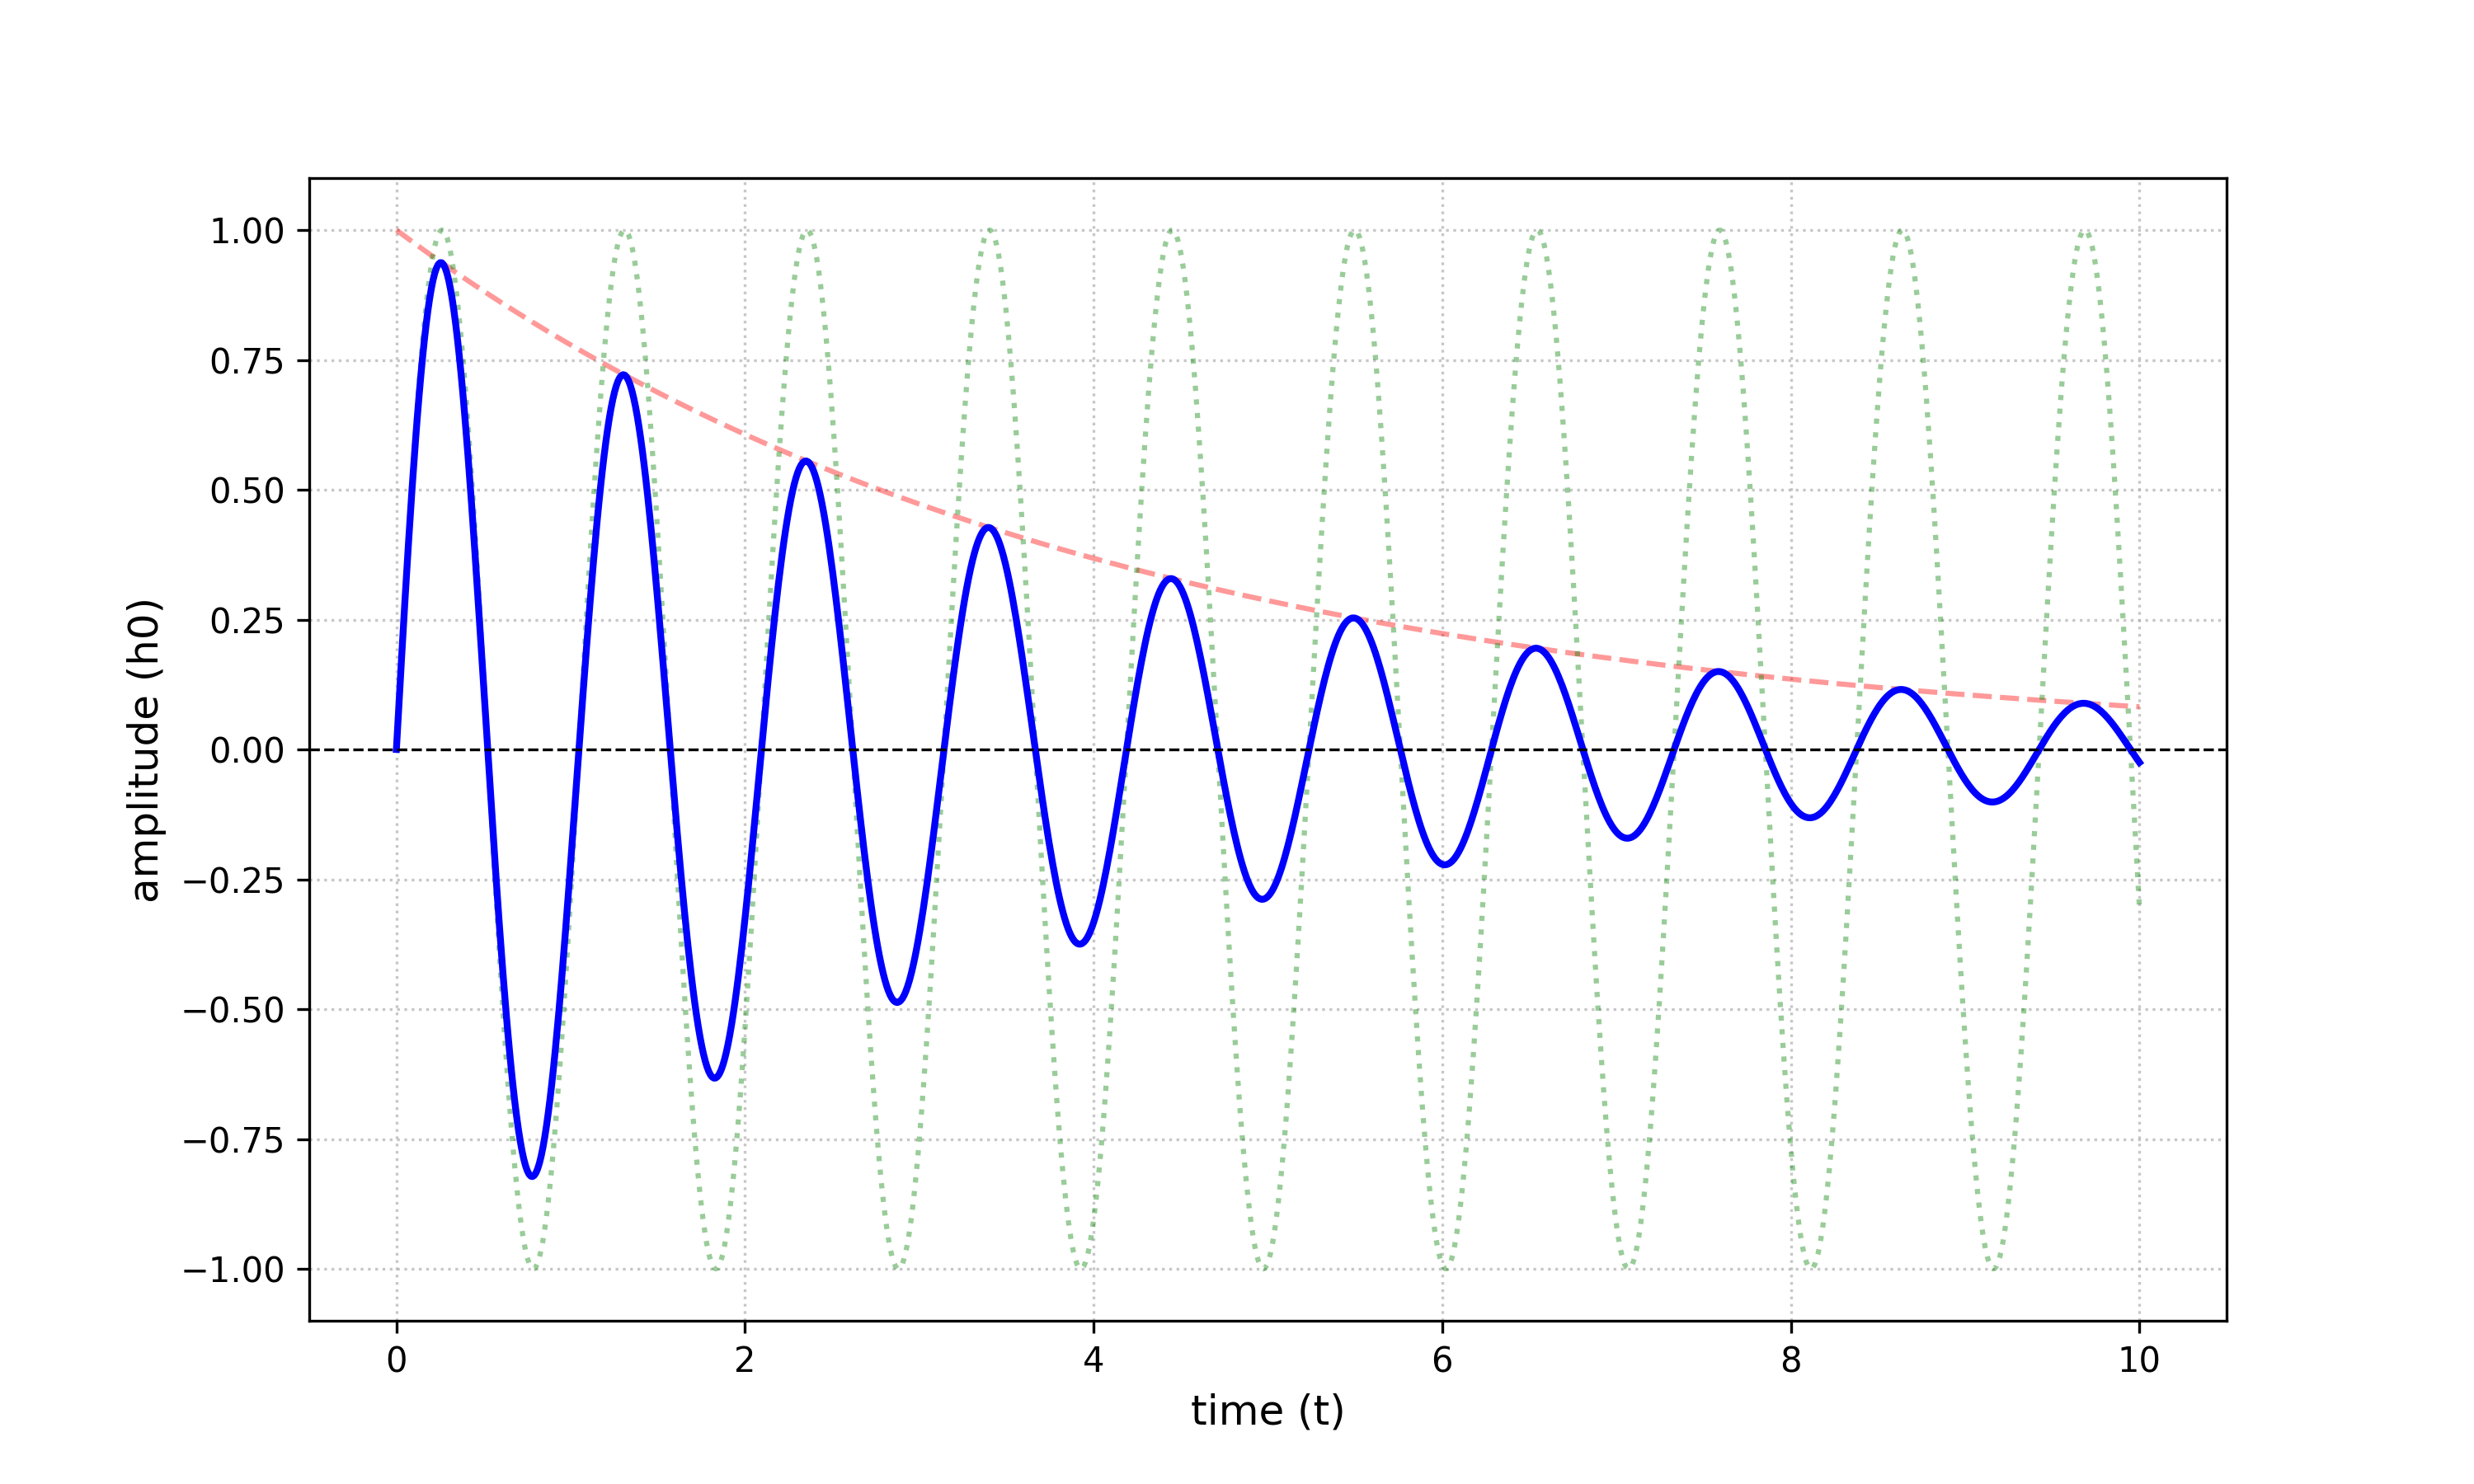
\includegraphics[width=\textwidth]{Figures/Flutter_Decay_Solution_Plot.png}
        \subcaption{Decay solution}
    \end{minipage}
    \hfill
    \begin{minipage}{0.48\textwidth}
        \centering
        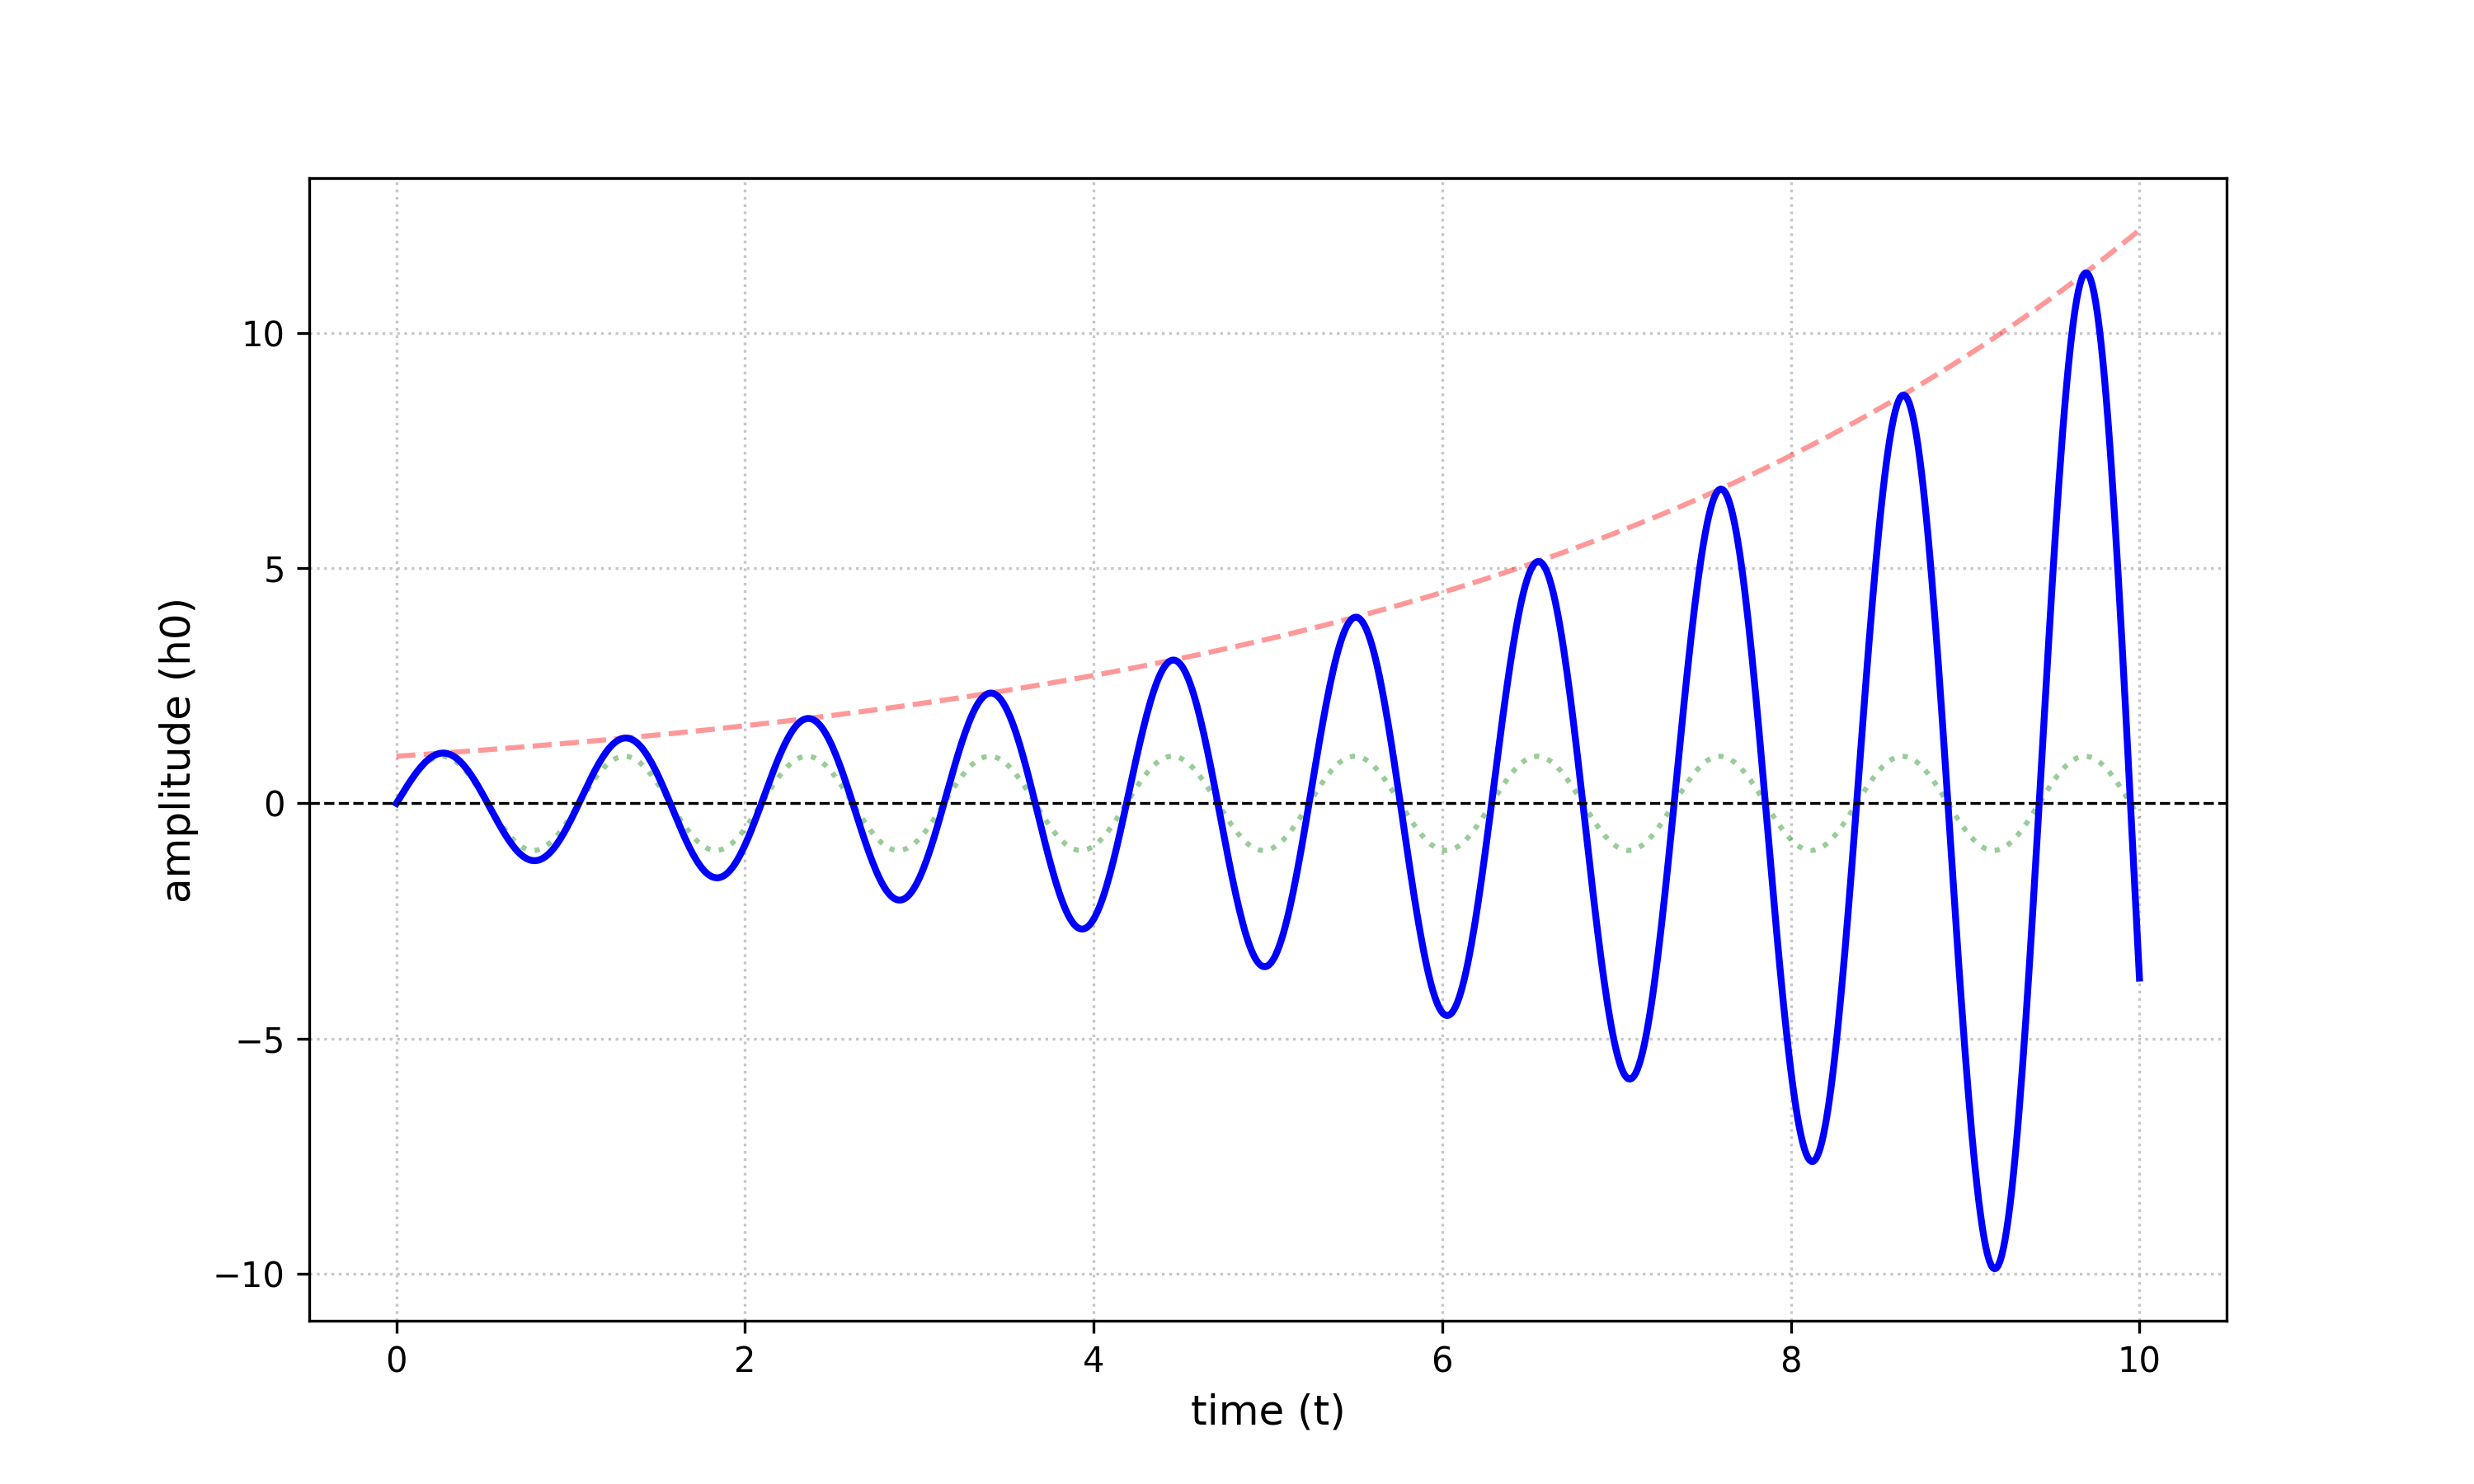
\includegraphics[width=\textwidth]{Figures/Flutter_Growth_Solution_Plot.png}
        \subcaption{Growth solution}
    \end{minipage}
    \caption{Time-domain response of the flutter/galloping solution}
    \label{fig:Flutter_Solution_Plot}
\end{figure}

A Python tool has been developed to solve this linearised eigenvalue problem and identify the critical wind speed. 
Determining the critical wind speed is an iterative process because the flutter derivatives are functions of reduced velocity, 
which in turn is a function of wind speed. Hence the following steps ( which forms the algorithm of the code) are 
performed iteratively to find the critical wind speed:

\begin{enumerate}
    \item A reduced velocity $U_r = U/(fB)$ is selected.
    \item Flutter derivatives corresponding to that reduced velocity are
          interpolated from the flutter-derivative functions.
    \item The linearised eigenvalue problem is solved for $\omega$.
    \item If the system is stable, the reduced velocity is increased
          and the process repeats until the system first becomes unstable.
          The critical wind speed is the speed at which $\omega_i$ changes sign from positive to negative, 
          indicating the onset of flutter instability.
    \item The actual critical wind speed is then recovered from
    \begin{equation}
        U_c = U_{r,c}\,\frac{\omega_r}{2\pi}\,B,
        \label{eq:Uc}
    \end{equation}
    where $U_{r,c}$ is the reduced critical velocity and $\omega_r$ is
    the real part of the eigenfrequency at that point.
\end{enumerate}


\end{document}